\documentclass[a4paper]{article}

\usepackage[T1]{fontenc}
%\usepackage[utf8]{inputenc}
\usepackage[italian]{babel}
\usepackage{amssymb}
\usepackage{hyperref}
\usepackage{mathtools}
\usepackage{amsthm}
\usepackage[ruled,vlined,noend]{algorithm2e}

%%%%%%%%%%%%%%%%%%%%%%%%%%%%%%%%%%%%
\usepackage{listings} 
\lstdefinestyle{mystyle}{
    breakatwhitespace=false,                   
    captionpos=b,                    
    keepspaces=true,                 
    numbers=left,                    
    numbersep=5pt,                  
    showspaces=false,                
    showstringspaces=false,
    showtabs=False,                  
    tabsize=2
}

\lstset{style=mystyle}

\usepackage{setspace}
\singlespacing

%%%%%%%%%%%%%%%%%%%%%%%%%%%%%%%%%%%%
\usepackage{ulem} 
\usepackage{soul}

\usepackage{graphicx}
\graphicspath{ {./images/} }
%%%%%%%%%%%%%%%%%%%%%%%%%%%%%%%%%%%%

\mathtoolsset{showonlyrefs}  
\hypersetup{
    colorlinks=true,
    linkcolor=black,
    filecolor=black,      
    urlcolor=black,
}

\newcommand{\pluseq}{\mathrel{{+}{=}}}

\newtheorem {theorem}{Theorem}
\newtheorem{corollary}{Corollary}
\newtheorem{lemma}{Lemma}
\newtheorem{remark}{Remark}
\newtheorem{definition}{Definition}

\setcounter{secnumdepth}{3}
\setcounter{tocdepth}{3}

\title{Advanced Programming}
\author{Federico Bruzzone}
%\date{}
\makeindex

\begin{document}
\maketitle
\newpage
% \setlength{\parskip}{0.15em}
\tableofcontents
\setlength{\parindent}{0pt}
\setlength{\parskip}{0.8em}
\newpage

%\section{section}
...

\subsection{subsection}
	
\paragraph{paragraph}

\begin{remark}
    ...
\end{remark}

\subsubsection{subsubsection}

\subsubsection{subsubsection}

\paragraph{paragraph}

\subsection{subsection}
...
\begin{enumerate}
    \item 
    \item
    \item 
\end{enumerate}

\begin{itemize}
	\item 
    \item 
\end{itemize}

\begin{theorem}
    $PO \subseteq NPO$
\end{theorem}
\begin{proof}
    ...
\end{proof}

\begin{equation}
    \begin{aligned}
        \mathit{APX} = \{\Pi | \Pi \mathit{\;di\;ottimizzazione\;t.c.\;}
\exists \rho \geq 1, A, \\\mathit{t.c\;} x\rightarrow A \rightarrow y(x)\;\mathit{con}\;R_\Pi(x, y) \leq \rho\}
    \end{aligned}
\end{equation}


\paragraph{Algoritmo di risoluzione}
L'algoritmo di risoluzione è abbastanza semplice e si basa sulla 
ricerca di un cammino aumentante.

\begin{algorithm}[H]
    \SetAlgoLined
    \KwIn{$G=(V,E)$}
    \KwResult{Matching $M$ per $G$}
     $M \gets \emptyset$\\
     \While{$\Pi = \mathit{findAugmenting(G)}$}{
        $M.update(\Pi)$
     }
     \Return{M}
     \caption{BiMaxMatching}
\end{algorithm}


\subsection{Tecniche greedy}
Nella sezione a seguire si presentano problemi di ottimizzazione per cui 
tecniche greedy funzionano abbastanza bene. 
I problemi affrontati sono quelli di \emph{Load Balancing}, \emph{Center Selection} e \emph{Set Cover}.

\subsubsection{Load balancing}
\label{lb}
Il problema di Load Balancing può essere visto come il compito
di assegnare a macchine dei lavori da compiere, che richiedono del tempo, 
in modo da minimizzare il tempo totale.


\begin{theorem}
    Load Balancing è NPO completo
\end{theorem}
Bisogna perciò trovare un modo di approssimare una soluzione.
\paragraph{Greedy balance}
Il primo approccio alla risoluzione del problema è quello di assegnare la prossima
task alla macchina più scarica in questo momento.

\begin{algorithm}[H]
    \SetAlgoLined
    \KwIn{$M$ numero di macchine, $t_0, \dots, t_n$ task}
    \KwResult{Assegnamento delle task alle macchine}
     $L_i \gets 0\;\forall i \in M$\\
     $\alpha \gets \emptyset$\\
     \For{$j = 0, \dots, n$}{
         $\hat{i} = \min(L_i)$\\
         $\alpha(j) = \hat{i}$\\
         $L_{\hat{i}} \pluseq t_j$
     }
     \Return{$\alpha$}
     \caption{GreedyBalance}
\end{algorithm}

\begin{lstlisting} %[language=Python, caption=Python example]

import numpy as np
    
def incmatrix(genl1,genl2):
    m = len(genl1)
    n = len(genl2)
    M = None #to become the incidence matrix
    VT = np.zeros((n*m,1), int)  #dummy variable
    
    #compute the bitwise xor matrix
    M1 = bitxormatrix(genl1)
    M2 = np.triu(bitxormatrix(genl2),1) 

    for i in range(m-1):
        for j in range(i+1, m):
            [r,c] = np.where(M2 == M1[i,j])
            for k in range(len(r)):
                VT[(i)*n + r[k]] = 1;
                VT[(i)*n + c[k]] = 1;
                VT[(j)*n + r[k]] = 1;
                VT[(j)*n + c[k]] = 1;
                
                if M is None:
                    M = np.copy(VT)
                else:
                    M = np.concatenate((M, VT), 1)
                
                VT = np.zeros((n*m,1), int)
    
    return M
\end{lstlisting}

%%%%%%%%%%%%%%%%%
\usepackage{listings}
\usepackage{xcolor}

\definecolor{codegreen}{rgb}{0,0.6,0}
\definecolor{codegray}{rgb}{0.5,0.5,0.5}
\definecolor{codepurple}{rgb}{0.58,0,0.82}
\definecolor{backcolour}{rgb}{0.95,0.95,0.92}

\lstdefinestyle{mystyle}{
    backgroundcolor=\color{backcolour},   
    commentstyle=\color{codegreen},
    keywordstyle=\color{magenta},
    numberstyle=\tiny\color{codegray},
    stringstyle=\color{codepurple},
    basicstyle=\ttfamily\footnotesize,
    breakatwhitespace=false,         
    breaklines=true,                 
    captionpos=b,                    
    keepspaces=true,                 
    numbers=left,                    
    numbersep=5pt,                  
    showspaces=false,                
    showstringspaces=false,
    showtabs=false,                  
    tabsize=2
}

\lstset{style=mystyle}
\section{Python}

\subsection{Python's whys \& hows}

\subsubsection{What is Python}
\textbf{Python is a general-purpose high-level programming language}
\begin{itemize}
	\item it pushes code readability and productivity;
	\item it best fits the role of scripting language.
	\end{itemize}
\textbf{Python support multiple programming paradigms}
\begin{itemize}
	\item imperative (function, state, ...);
	\item object-oriented/based (objects, methods, inheritance, ...);
	\item functional (lambda abstractions, generators, dynamic typing, ...).
\end{itemize}
\textbf{Python is}
\begin{itemize}
	\item interpreted, dynamic typed and object-based;
	\item open-source.
\end{itemize}

\subsubsection{How to use Python}	
\textbf{We are condidering Python 3+}
\begin{itemize}
	\item version > 3 is incompatible with previus version;
	\item version 2.7 is the current version.
\end{itemize}
\textbf{A python program can be:}
\begin{itemize}
	\item edited in the python shell and executed step-by-step by the shell;
	\item edited and run through the iterpreter.
\end{itemize}

\subsection{Overview of the Basic Concepts}	

\subsubsection{Our first Python program}
\hrule
\begin{lstlisting}[language=Python, caption=humanize.py]
SUFFIXES = {1000: ['KB', 'MB', 'GB', 'TB', 'PB', 'EB', 'ZB', 'YB'], 
            1024: ['KiB', 'MiB', 'GiB', 'TiB', 'PiB', 'EiB', 'ZiB', 'YiB']}
def approximate_size(size, a_kilobyte_is_1024_bytes=True):
	''' Convert a file size to human-readable form. '''
	if size < 0:
		raise ValueError('number must be non-negative')
	multiple = 1024 if a_kilobyte_is_1024_bytes else 1000
	for suffix in SUFFIX[multiple]:
		size /= multiple
		if size < multiple:
			return '{0:.1f} {1}'.format(size, suffix)
		raise ValueError('number too large')
				
if __name__ == '__main__':
	print(approximate_size(1000000000000, False))
	print(approximate_size(1000000000000))
\end{lstlisting}
\hrule	

\subsubsection{Declaring function}	
\textbf{Python has function}
\begin{itemize}
	\item no header files à la C/C++;
	\item no interface/implementation à la Java.
\end{itemize}			
\hrule
\begin{lstlisting}[language=Python]
def approximate_size(size, a_kilobyte_is_1024_bytes=True):
\end{lstlisting}	
\begin{enumerate}
	\item \textbf{def}: function definition keyword;
	\item \textbf{approximate\_size}: function name;
	\item \textbf{a\_kilobyte\_is\_1024\_bytes}: comma separate argument list;
	\item \textbf{=True}: default value.
\end{enumerate}
\hrule		
\textbf{Python has function}
\begin{itemize}
	\item no return type, it always return a value (\textbf{None} as a default); 
	\item no parameter types, the interpreter figures out the parameter type.
\end{itemize}	

\subsubsection{Calling Functions}
\textbf{Look at the bottom of the \textit{humanize.py} program}
\hrule
\begin{lstlisting}[language=Python]
if __name__ == '__main__':
	print(approximate_size(1000000000000, False))
	print(approximate_size(1000000000000))
\end{lstlisting}
\begin{enumerate}
	\item[2] in this call to \textbf{approximate\_size()}, the \textbf{a\_kilobyte\_is\_1024\_bytes} parameter will be \textbf{False} since you explicitly pass it to the function;
	\item[3] in this row we call  \textbf{approximate\_size()} with only a value, the parameter \textbf{a\_kilobyte\_is\_1024\_bytes} will be \textbf{True} as defined in the function declaration.
\end{enumerate}
\hrule
\textbf{Value can be passed by name as in}:
\hrule
\begin{lstlisting}[language=Python]
def approximate_size(a_kilobyte_is_1024_bytes=True, size=1000000000000)
\end{lstlisting}	
\hrule
\textbf{Parameters' order is not relevant}

\subsubsection{Writing readable code}
\textbf{Documentation Strings}
A python function can be documented by a documentation string (docstring for short).
\begin{center}
	\textit{''' Convert a file size to human-readable form.  '''}
\end{center}
\textbf{Triple quotes delimit a single multi-string}
\begin{itemize}
	\item if it immediatly follows the function's declaration it is the doc-string associated to the function;
	\item docstrings can be retrieved at run-time (they are attributes).
\end{itemize}
\textbf{Case-Sensitive}
All names in Python are case-sensitive

\subsubsection{Everything is an object}
\textbf{Everything in Python is an object, functions included}
\begin{itemize}
	\item \textbf{import} can be used to load python programs in the system as modules;
	\item the dot-notation gives access to the the public functionality of the imported modules;
	\item the dot-notation can be used to access the attributes (e.g., the \textbf{\_\_doc\_\_})
	\item \textbf{humanize\.approximate\_size.\_\_doc\_\_} gives access to the docstring of the \textbf{approximate\_size()} function; the docstring is stored as an attribute.
\end{itemize}

\subsubsection{Everything is an object (Cont'd)}
\textbf{In python is an object, better, is a \textbf{first-calss object}}
\begin{itemize}
	\item everything can be assigned to a variable or passed as an argument
\end{itemize}
\hrule
\begin{lstlisting}[language=Python]
h1 = humanize.approximate_size(9128)
h2 = humanize.approximate_size
\end{lstlisting}	
\begin{itemize}
	\item \textbf{h1} contains the string calculated by \textbf{approximate\_size(9128};
	\item \textbf{h2} contains the "function" object \textbf{approximate\_size()}, the result is not calculated yet;
	\item to simplify the concept: \textbf{h2} can be considered as a new name of (alias to) \textbf{approximate\_size}.
\end{itemize}
\hrule

\subsubsection{Indenting code}
\textbf{No explicit block delimiters}
\begin{itemize}
	\item the only delimiter is a column (':') and the code indentation;
	\item code blocks (e.g., functions, if statements, loops, ...) are defined by their indentation;
	\item white spaces and tabs are relevant: use them consistently;
	\item indentation is checked by the compiler.
\end{itemize}

\subsubsection{Exceptions}
\textbf{Exceptions are Anomaly Situations}
\begin{itemize}
	\item C encourages the use of return codes which you check;
	\item Python encourages the use of exceptions which you handles.
\end{itemize}
\textbf{Raising Exceptions}
\begin{itemize}
	\item the \textbf{raise} statement is used to rise an exception as in:
\begin{lstlisting}[language=Python]
raise ValueError('number must be non-negative')
\end{lstlisting}
	\item syntax recalls function calls: \textbf{raise} statement followed by an exception name with an optional argument;
	\item exceptions are relized by classes.
\end{itemize}
\textbf{No need to list the exceptions in the function declaration handling Exceptions}
\begin{itemize}
	\item an exception is handled by a \textbf{try} ... \textbf{except} block.
\hrule
\begin{lstlisting}[language=Python]
try:
	from lxml import etree
except ImportError:
	import xml.etree.ElementTree as etree
\end{lstlisting}
\hrule
\end{itemize}

\subsubsection{Running scripts}
\textbf{Look again, at the bottom of the \textit{humanize.py} program}:
\hrule
\begin{lstlisting}
if __name__ == '__main__':
	print(approximate_size(1000000000000, False))
	print(approximate_size(1000000000000))
\end{lstlisting}
\hrule
\textbf{Modules are Objects}
\begin{itemize}
	\item they have a built-in attribute \textbf{\_\_name\_\_}
\end{itemize}
\textbf{The value of \textbf{\_\_name\_\_} depends on how you call it}
\begin{itemize}
	\item if imported it contains the name of the file without path and extension.
\end{itemize}

\section{Primitive Datatypes \& recursion in Python}

Python's Native Datatypes

\subsection{Primitive types}

\subsubsection{Introduction}
In python \textbf{every value has a datatype}, but you do not need to declare it.

\textbf{How does that work?}

Based on each variable's assignment, python figures out what type it is and keeps tracks of that internally.

\subsubsection{Boolean}
Python provides two constants

- \textbf{True} and \textbf{False}

\textbf{Operations on Booleans}

Logic operations: \textit{and} \textit{or} \textit{not}

Relational operators: \textit{==} \textit{!=} \textit{<} \textit{>} \textit{<=} \textit{>=}

Note that python allows chains of comparisons
\begin{lstlisting}[language=Python]
>>> x = 3
>>> 1<x<=5
> True
\end{lstlisting}

\subsubsection{Number}
\textbf{Two kinds of number: integer and floats}
\begin{itemize}
	\item no class declaration to distinguish them
	\item they can be distiguished by the presence/absence of the decimal point
\begin{lstlisting}[language=Python]
>>> type(1)
> <class 'int'>
>>> isinstance(1, int)
> True
>>> 1+1
> 2
>>> 1+1.0
> 2.0
>>>type(2.0)
> <class 'float'>
\end{lstlisting}
	\item \textbf{type()} function provides the type of any value or variable;
	\item \textbf{isinstance()} check if a value or variable is of a given type;
	\item adding an int to an yields another int but adding it to a float yields a float.
\end{itemize}

\subsubsection{Operations on numbers}
\textbf{Coercion \& size}
\begin{itemize}
	\item \textbf{int()} function truncates a gloat to an integer;
	\item \textbf{float()} function promotes an integer to a float;
	\item integers can be arbitrarly large;
	\item float are accurate to 15 decimal places.
\end{itemize}
\textbf{Operators} (just a few)

\textit{+} \textit{-}

\textit{*} \textit{**}

\textit{/} \textit{//} \textit{\%}

\subsection{Collection}

\subsubsection{Lists}
\textbf{A python list looks very closely to an array}
\begin{itemize}
	\item direct access to the members through [];
\begin{lstlisting}[language=Python]
>>> a_list = ['1', 1, 'a', 'example']
>>> type(a_list)
> <class 'list'>
\end{lstlisting}
\end{itemize}
\textbf{But}
\begin{itemize}
	\item negative numbers give access ti the members backwards, e.g., \textbf{a\_list[-2] == a\_list[4-2] == a\_list[2]};
	\item the list is not fixed in size;
	\item the members are not homogeneous.
\end{itemize}

\subsubsection{Lists: Slicing a List}
A slice og a list can be yielded by the [:] operator and specifying the position of the first item you want in the slice and of the first you want to exclude

\begin{lstlisting}[language=Python]
>>> a_list = [1, 2, 3, 4, 5]
>>> a_list[1:3]
> [2, 3]
>>> a_list[:-2]
> [1, 2, 3]
>>> a_list[2:]
> [3, 4, 5]
\end{lstlisting}

Note that omitting one of the two indexes you get respectively the first and the last item in tbe list.

\subsubsection{Lists: Adding items into the list}
\textbf{Four ways}
\begin{itemize}
	\item \textbf{+} operator concatenates two lists;
	\item \textbf{append()} method append an item to the end of the list;
	\item \textbf{extend()} method appends a list to the end of the list
	\item \textbf{insert()} method appends an item at given position.
\end{itemize}

\subsubsection{Lists: Introspecting on the list}
\textbf{You can check if an element is in thelist}
\begin{lstlisting}[language=Python]
>>> a_list = [3,14, 1, 'c', 3.14]
>>> 3.14 in a_list
> True
\end{lstlisting}
\textbf{Count the number of occurrences}
\begin{lstlisting}[language=Python]
>>> a_list.count(3.14)
> 2
\end{lstlisting}
\textbf{Look for an item position}
\begin{lstlisting}[language=Python]
>>> a_list.index(3.14)
> 1
\end{lstlisting}
\textbf{Elements can be removed by}
\begin{itemize}
	\item position
\begin{lstlisting}[language=Python]
>>> del a_list[2]
>>> a_list
> [3,14, 1, 3.14]
\end{lstlisting}
	\item value
\begin{lstlisting}[language=Python]
>>> a_list.remove(3.14)
>>> a_list
> [3,14, 1]
\end{lstlisting}
\end{itemize}
In both cases the list is compacted to fill the gap.

\subsubsection{Tuples}
\textbf{Tuples are immutable lists.}
\begin{lstlisting}[language=Python]
>>> a_tuple = (3,14, 1, 'c', 3.14)
>>> a_tuple
> (3,14, 1, 'c', 3.14)
>>> type(a_tuple)
> <class 'tuple'>
\end{lstlisting}
\textbf{As a list}
\begin{itemize}
	\item parenthesis instead of square brackets;
	\item ordered set with direct access to the elements through the position;
	\item negative indexes count backward.
\end{itemize}
\textbf{On the contrary}
\begin{itemize}
	\item no \textbf{append()}, \textbf{extend()}, \textbf{insert()}, \textbf{remove()} and so on.
\end{itemize}

\subsubsection{Tuples (Cont'd)}
\textbf{Multiple assignments}
Tuple can be used for multiple assignments and to return multiple values.
\begin{lstlisting}[language=Python]
>>> a_tuple = (1, 2)
>>> (a,b) = a_tuple
>>> a
> 1
>>> b
> 2
\end{lstlisting}
\textbf{Benefits}
\begin{itemize}
	\item tuples are faster than lists;
	\item tuples are safer than lists;
	\item tuples can be used as keys for dictionaries.
\end{itemize}

\subsubsection{Sets}
\textbf{Sets are unordered "bags" of unique values.}
\begin{lstlisting}[language=Python]
>>> a_set = {1, 2}
>>> a_set
> {1, 2}
>>> len(a_set)
> 2
>>> b_set = set()
>>> b_set
> set() ''' empty set '''
\end{lstlisting}
\textbf{A set can be created out of a list}
\begin{lstlisting}[language=Python]
>>> a_list = [1, 'a', 3.14, "a string"]
>>> a_set = set(a_list)
>>> a_set
> {'a', 1, 'a string', 3.14}
\end{lstlisting}

\subsubsection{Sets: Modifying a set}
\textbf{Adding elements to a set}
\begin{lstlisting}[language=Python]
>>> a_set = set()
>>> a_set.add(7)
>>> a_set.add(3)
>>> a_set
> {3, 7}
>>> a_set.add(7)
>>> a_set
> {3, 7}
\end{lstlisting}
Sets do not admit duplicates so to add a value twice has no effects.
\textbf{Union of sets}
\begin{lstlisting}[language=Python]
>>> b_set = {3, 5, 3.14, 1, 7}
>>> a_set.update(b_set)
>>> a_set
> {1, 3, 5, 7, 3.14}
\end{lstlisting}

\subsubsection{Dictionaries}
\textbf{A dictionary is an unordered set of key-value pairs}
\begin{itemize}
	\item when you add a key to the dictionary you must also add a value for that key;
	\item a value for a key can be chenged at any time.
\end{itemize}
\textbf{The syntax is similar to stes, but}
\begin{itemize}
	\item you list comma separate couples of key/value;
	\item {} is the empty dictionary.
\end{itemize}
Note that you cannot have more than one entry with the same key.

\subsection{String}
\subsubsection{String}
\textbf{Python's string are a sequence of unicode characters}
\textbf{String behave as lists: you can:}
\begin{itemize}
	\item get the string length with the \textbf{len} function;
	\item concatenate string with the \textbf{+} operator;
	\item slicing works as well.
\end{itemize}
Note that ", ' and ''' (three-in-a-row qoutes) can be used to define a string constant.

\subsubsection{Formatting string}
\textbf{Python 3 support formatting values into strings.}

that is, to insert a value into a string with a placeholder.

\textbf{Looking back at the \textit{humanize.py} example}
\begin{lstlisting}[language=Python]
for suffix in SUFFIX[multiple]:
		size /= multiple
		if size < multiple:
			return '{0:.1f} {1}'.format(size, suffix)
		raise ValueError('number too large')
\end{lstlisting}
\begin{itemize}
	\item  \textbf{\{0\}}, \textbf{\{1\}}, ... are placeholders that are replaced by the arguments of \textbf{format()}
	\item  \textbf{:.lf} is a format specifier, itcan be used to add space-padding, align strings, control decimal precision and convert number to hexadecimal as in C.
\end{itemize}

\subsubsection{Bytes}
\textbf{An immutable sequence of numbers (0-255) is a bytes object.}

\textbf{The byte literal syntax (b'') is used to define a bytes object}

Each byte within the byte literal can be an ascii character or an encoded hexadecimal number from x00 to xff 

\subsection{Recursion}
\subsubsection{Definition: Recursive function}
A function is called recursive when it is defined through itself.

Example: Factorial.
\begin{itemize}
	\item 5! = 5*4*3*2*1
	\item Note that: 5! = 5*4!, 4! = 4*3! and so on.
\end{itemize}
Potentially a recursive computation

From the mathematical definition:
\begin{lstlisting}
n! = 
1        if n=0
n*(n-1)! otherwise
\end{lstlisting}

When n=0 is the base of the recursive computation (axiom) whreas the second step is the inductive step.

\subsubsection{What in python?}
Still, a function is recursive when its execution implies another invocation to itself.
\begin{itemize}
	\item directly, e.g., in the function body there is an explicit call to itself;
	\item indirectly, e.g., in the function calls another function that calls the function itself.
\end{itemize}

\begin{lstlisting}
def fact(n):
	return 1 if n<=1 else n*fact(n-1)
	
if __name__ == __main__:
	for i in [5, 7, 15, 25, 30, 42, 100]:
		print('fact({0:3d}) :- {1}'.format(i, fact(i)))
\end{lstlisting}

\subsubsection{Execution: What's happen?}
Still, a function is recursive when its execution implies another invocation to itself.
\begin{itemize}
	\item directly, e.g., in the function body there is an explicit call to itself;
	\item indirectly, e.g., in the function calls another function that calls the function itself.
\end{itemize}

\begin{lstlisting}
def fact(n):
	return
		1
		if <=1
		else n*fact(n-1)
\end{lstlisting}

\textbf{It runs fact(4):}
\begin{itemize}
	\item a new frame with n=4 is pushed on the stack;
	\item n is greater than 1;
	\item it calculates 4*fact(3).
\end{itemize}
\textbf{It runs fact(3):}
\begin{itemize}
	\item a new frame with n=3 is pushed on the stack;
	\item n is greater than 1;
	\item it calculates 3*fact(2).
\end{itemize}
\textbf{It runs fact(2):}
\begin{itemize}
	\item a new frame with n=2 is pushed on the stack;
	\item n is greater than 1;
	\item it calculates 2*fact(1).
\end{itemize}
\textbf{It runs fact(1):}
\begin{itemize}
	\item a new frame with n=2 is pushed on the stack;
	\item n is equal to 1;
	\item it returns 1.
\end{itemize}

\subsubsection{Iteration is more efficient}
The iterative implementation is more efficient...

The overhead is mainly due to the creation of the frame but this also affects the occupied memory.

As an example, the call fibo(1000)
\begin{itemize}
	\item gives an answer if calculated by the iterative implementation;
	\item raises a RuntimeError Exception in the recursive solution.
\end{itemize}
\section{Comprehensions}

\subsection{Playing around with...}

\subsubsection{Implementing the LS command}

\begin{lstlisting}[language=Python]
import os, sys, time, humanize
from start imoprt *

modes = { 
	'r': (S_IXUSR,S_IXGRP,S_IXOTH), 
	'w': (S_IXUSR,S_IXGRP,S_IXOTH), 
	'x': (S_IXUSR,S_IXGRP,S_IXOTH)
}

def format_mode(mode):
	s = 'd' if S_ISDIR(mode) else "-"
	for i in range(3):
		for j in ['r', 'w', 'x']:
			s += j if S_ISDIR(mode) & modes[i][j] else '-'
	return s
	
def formate_date(date):
	d = time.localtime(date)
	return "{0:4}-{1:02d}-{2:02d} {3:02d}:{4:02d}:{5:02d}".format(
          d.tm_year, d.tm_mon, d.tm_mday, d.tm_hour, d.tm_min, d.tm_sec)

def ls(dir):
	print("List of {0}:".format(dir))
	for file in os.listdir(dir):
		metadata = os.stat(file)
		print("{2} {1:6} {3} {0} ".format(
		      file, approximate_size(metadata.st_size, False),
		      format_mode(metadata.st_mode), format_date(metadata.st_ntime)))

if __name__ == "__main__": ls(sys.argv[1])
\end{lstlisting}

\subsection{Introduction}
\textbf{Comprehensions are a compact way to transfor a set of data into another}
\begin{itemize}
	\item it applies to mostly all python's structure sype, e.g., lists, sets, dictionaries;
	\item it is in contrast to list all the elements.
\end{itemize}

\textbf{Some basic comprehensions applied to lists, stes and dictionaries respectively}
\begin{itemize}
	\item a list composed of the first ten integers
\begin{lstlisting}[language=Python]
>>> [elem for elem in range (1, 11)]
> [1, 2, 3, 4, 5, 6, 7, 8, 9, 10]
\end{lstlisting}
	\item a set composed of the first ten even integers
\begin{lstlisting}[language=Python]
>>> {elem*2 for elem in range (1, 11)}
> {2, 4, 6, 8, 10, 12, 14, 16, 18, 20}
\end{lstlisting}
	\item a dictionary composed of the first ten couples (n, n\^2)
\begin{lstlisting}[language=Python]
>>> {elem:elem*2 for elem in range (1, 11)}
> {1: 1, 2: 4, 3: 9, 4: 16, 5: 25, 6: 36, 7: 49, 8: 64, 9: 81, 10: 100}
\end{lstlisting}
\end{itemize}

\subsection{To filter out elemets of a dataset}
\textbf{Comprehensions can reduce the elements in the dataset after a constrint.}

\textbf{E.g., to select perfect squares out of the first 100 integers}
\begin{lstlisting}[language=Python]
>>> [elem for elem in range(1, 101) if(int(elem**.5))**2 == elem]
> [1, 4, 9, 16, 25, 36, 49, 64, 81, 100]
\end{lstlisting}
\begin{itemize}
	\item \textbf{range(1,101)} generates a list of the first 100 integers (first extreme included, second excluded);
	\item the comprehension skims through the list selecting those elemetns whose square of the integral part of its square roots are equal.
\end{itemize}
\textbf{E.g., to select the odd numbers out of a tuple}
\begin{lstlisting}[language=Python]
>>> {x for c in (1, 22, 31, 23, 10, 11, 11, -1, 34, 76, 778, 10101, 5, 44) 
     if x%2 != 0}
> {1, 31, 23, 11, -1, 10101, 5}
\end{lstlisting}
\begin{itemize}
	\item note that the second 11 is removed from the set;
	\item the set does note respect the tuple order (it is not ordered at all).
\end{itemize}

\subsection{To select multiple values}
\textbf{Comprehensions can select multiple values out of the dataset.}

\textbf{E.g., to swap key and value in the dictionary}
\begin{lstlisting}[language=Python]
>>> a_dict = {'a': 1, 'b': 2, 'c': 3}
>>> {value:key for key, value in a_dict.items()}
> {1: 'a', 2: 'b', 3: 'c'}
\end{lstlisting}
\textbf{Comprehensions can select values out of multiple datasets.}

\textbf{E.g., to merge two sets in a set of couples}
\begin{lstlisting}[language=Python]
>>> english = ['a', 'b', 'c'}
>>> greek = [$\alpha$, $\beta$, $\gamma$]
>>> [(english[i], greek[i]) for i in range(0, len(english))]
> [('a', $\alpha$), ('b', $\beta$), ('c', $\gamma$)]
\end{lstlisting}


\textbf{E.g., to calculate the cartesian product}
\begin{lstlisting}[language=Python]
>>> {(x,y) for x in range(3) for y in range (5)}
> {(0,1),(1,2),(0,0),(2,2),(1,1),(1,4),(0,2),(2,0),
(1,3),(2,3),(2,1),(0,4),(2,4),(0,3),(1,0)}
\end{lstlisting}

\subsection{Comprehensions @ work: prime numbers calculation}
\textbf{Classic approach to the prime numbers calculation}
\begin{lstlisting}[language=Python]
def is_prime(x):
	div = 2
	while div <= math.sqrt(x):
		if x%div == 1: return False		
		else: div += 1
	return True

if __name == "__main__":
	primes = []
	for i in range(1, 50):
		if is_prime(i): primes.append(i)
	print(primes)
\end{lstlisting}
\textbf{The alsorithm again but using comprehensions}
\begin{lstlisting}[language=Python]
def is_prime(x):	
	div = [elem for elem in range(0, math.sqrt(x)) if x%elem==0]
	return len(div) == 0

if __name == "__main__":
	print([elem for elem in range(1,50) if is_prime(elem)])
\end{lstlisting}

\subsection{Comprehensions @ work: quicksort}
\begin{lstlisting}[language=Python]
def quicksort(s):
	if len(s) == 0: return []
	else
		return quicksort([x for x in s[1:] if x < s[0]]) + 
		[s[0]] + 
		quicksort([s for x in s[1:] if x >= s[0]])

if __name__ == "__main__":
	print(quicksort([])
	print(quicksort([2, 4, 1, 3, 5, 8, 6, 7,])
	print(quicksort("pineapple")
	print(''.join(quicksort('pineapple)))
\end{lstlisting}

\begin{lstlisting}[language=Python]
> []
> [1, 2, 3, 4, 5, 6, 7, 8]
> ['a', 'e',, 'e', 'i', 'l', 'n', 'p', 'p', 'p']
> aeeeilnppp
\end{lstlisting}




\section{Functional programming in Python}

\subsection{Functional programming}

\subsubsection{Overvirew}

\textbf{What is functional programming?}
\begin{itemize}
	\item Functions are first class (objects).

That is, everything you can do with "data" can be done with functions themselves (such as passing a function to another function).

	\item Recursion is used as a primary control structure.

In some languages, no other "loop" construct exists.

	\item There is focus on \textbf{list processing}.

Lists are often used with recursion on sub-lists as substitute for loops.

	\item "Pure" functional languages eschew side-effects.
	
This excludes assignments to track the program state.

This discorages the use of statements in favor of expression evaluations.
\end{itemize}

\textbf{Whys}

\begin{itemize}
	\item All these characteristics make for more rapidly developed, shorter, and less bug-prone code.
	\item A lot easier to prove formal properties of functional languages and programs than of imperative languages and programs.
\end{itemize}

\subsection{Functional programming in Python}

\subsubsection{map(), filter() \& reduce()}

\textbf{Python has functional capability since its first release}
with new  releases just a few syntactical sugar has been added

\textbf{Basic elements of functional programming in python are:}
\begin{itemize}
	\item \textbf{map()}: it applies a function to a sequence.
\begin{lstlisting}[language=Python]
>>> import math
>>> print(list(map(math.sqrt, [x**2 for x in range(1,11)])))
> [1.0, 2.0, 3.0, 4.0, 5.0, 6.0, 7.0, 8.0, 9.0, 10.0]
\end{lstlisting}
	\item \textbf{filter()}: it extracts from a list those elements which verify the passed function.
\begin{lstlisting}[language=Python]
>>> def odd(x): return (x%2 != 0)
>>> print(list(filter(odd, range(1,30))))
> [1, 3, 5, 7, 9, 11, 13, 15, 17, 19, 21, 23, 25, 27, 29]
\end{lstlisting}
\item \textbf{reduce()}: it reduces a list to a single element according to the passed funcion.
\begin{lstlisting}[language=Python]
>>> import functools
>>> def sum(x,y): return x+y
>>> print(functools.reduce(sum, range(1000)))
> 499500
\end{lstlisting}
\end{itemize}

Note, \textbf{map()} and \textbf{filter()} return an iterator rather than a list.

\subsubsection{Eliminating flow control statements: if}
\textbf{Short-circuit conditional call instead of if}
\begin{lstlisting}[language=Python]
def cond(x):
	return (x==1 and 'one') or (x==2 and 'two') or 'other'

def cond2(x):
	return ('one' and x==1) or ('two' and x==2) or 'other'

if __name__ == "__main__":
	for i in range(3):
		print("cond({0}) :- {1}".format(i, cond(i)))
	for i in range(3):
		print("cond2({0}) :- {1}".format(i, cond2(i)))
\end{lstlisting}
\begin{lstlisting}[language=Python]
> cond(0) :- other
> cond(1) :- one
> cond(2) :- two

> cond2(0) :- other
> cond2(1) :- True
> cond2(2) :- True
\end{lstlisting}

\textbf{Doing some abstraction}
\begin{lstlisting}[language=Python]
block = lambda s: s
cond = lambda x: (x==1 and block('one')) or 
                 (x==2 and block('two')) or 
                 block('other')

if __name__ == "__main__":
	print("cond({0}) :- {1}".format(3, cond(3)))
\end{lstlisting}
\begin{lstlisting}[language=Python]
> cond(3) :- other
\end{lstlisting}


\subsubsection{Do abstraction: Lambda functions}
The name lambda comes from lambda-calculus which uses the greek letter lambda to represent a similar comncept.

Lambda is a term used to refer to an \textbf{anonymous function}.
\begin{itemize}
	\item that is, a block of code which can be executed as if it were a function but without a name.
\end{itemize}

Lambdas can be defined anywhere a legal expression can occur.

A lambda looks like this:
\begin{lstlisting}[language=Python]
lambda "args": "an expr on the argss"
\end{lstlisting}

Thus the previous \textbf{reduce()} example could be rewritten as:
\begin{lstlisting}[language=Python]
>>> import functools
>>> print(functools.reduce(lambda i,j: i+x, range(10000)))
> 499500
\end{lstlisting}
Alternatively the lambda can assigned to a variable as in:
\begin{lstlisting}[language=Python]
>>> add = lambda i,j: i+j
>>> print(functools.reduce(add, range(10000)))
> 499500
\end{lstlisting}

\subsubsection{Envolving factorial}

\textbf{Traditional implementation}
\begin{lstlisting}[language=Python]
def fact(n):
	return 1 if n <= 1 else n*fact(n-1)
\end{lstlisting}
\textbf{Short-circuit implementation}
\begin{lstlisting}[language=Python]
def ffact(n):
	return (n <= 1 and 1) or n*ffact(n-1)	
\end{lstlisting}
\textbf{reduce()-based implementation}
\begin{lstlisting}[language=Python]
from functools import reduce
def f2fact(p):
	return reduce(lambda n,m: n*m, range(1, p+1))
\end{lstlisting}

\subsubsection{Eliminating flow control statements: sequence}

\textbf{Sequential program flow is typical of imperative programming}
it basically relies on side-effect (variable assignments)

\textbf{This is basically in contrast with the functional approach.}

\textbf{In a list processing style we have:}
\begin{lstlisting}[language=Python]
# let's create an execution utility function
do_it = lambda f: f()
# let f1, f2, f3 (etc) be functions that perform actions
map(do_it, [f1, f2, f3])
\end{lstlisting}
\begin{itemize}
	\item single statements of the sequence are replaced by funcions
	\item the sequene is realized by mapping an activation function to all the function objects that should compose the sequence.
\end{itemize}

\subsubsection{Eliminating while statements: Echo}

\textbf{Statement-based echo function}
\begin{lstlisting}[language=Python]
def echo_IMP():
	while True:
		x = input("FP -- ")
		if x == 'quit': break
		else: print(x)
		
if __name__ == "__main__": echo_IMP()
\end{lstlisting}

\textbf{First step toward a functional solution}
\begin{itemize}
	\item No print
	\item Utility function for "identity with side-effect" (a monad)
\end{itemize}
\begin{lstlisting}[language=Python]
def monadic_print(x)
	print(x)
	return x
\end{lstlisting}

\textbf{Functional version of the echo function}
\begin{lstlisting}[language=Python]
echo_FP = 
	lambda : monodic_print(input("FP -- ")=='quit' or echo_FP())

if __name__ == "__main__": echo_FP()
\end{lstlisting}

\subsubsection{Whys}

\textbf{Why? To eliminate the side-effects}
\begin{itemize}
	\item mostly all errors depend on variables that obtain unexpected values.
	\item functional programs bypass the issue by not assigning values to variables at all.
\end{itemize}

\textbf{E.g., To determine the pairs whose product is >25}
\begin{lstlisting}[language=Python]
def bigmuls(xs,ys):
	bigmuls = []
	for x in xs:
		for y in ys:
			if x*y > 25:
				bigmuls.append((x,y))
	return bigmuls
	
if __name__ == "__main__":
print(bigmuls((1,2,3,4),(10,15,3,22)))
\end{lstlisting}

 
\begin{lstlisting}[language=Python]
from functools import reduce
import itertools

bigmuls = lambda xs, ys: [x_y for x_y in
						  combine(xs,ys) if x_y[0]*x_y[1] > 25]
						  
combine = lambda xs, ys: itertools.zip_longest(
			             xs*len(ys), dupelms(ys,len(xs)))
			             
dupelms = lambda lst, n: reduce(lambda s, t: s+t,
                                list(map(lambda l,n=n: [l]*n, lst)))
                                
if __name__ == "__main__":
print(bigmuls([1,2,3,4],[10,15,3,22]))
\end{lstlisting}

\subsubsection{Future of map(), reduce() \& filter()}
\textbf{The future of the python's map(), filter(), and reduce is uncertain.}

\textbf{Comprehensions can easily replace map() and filter()}

\begin{itemize}
	\item \textbf{map()} can be replaced by
\begin{lstlisting}[language=Python]
>>> import math
>>> [math.sqrt(x**2) for x in range(1,11)]
> [1.0, 2.0, 3.0, 4.0, 5.0, 6.0, 7.0, 8.0, 9.0, 10.0]
\end{lstlisting}
	\item \textbf{filter()} can be replaced by
\begin{lstlisting}[language=Python]
>>> def odd(x): return (x%2 != 0)
>>> [x for x in range(1,30) if odd(x)]
[1, 3, 5, 7, 9, 11, 13, 15, 17, 19, 21, 23, 25, 27, 29]
\end{lstlisting}
\end{itemize}

Guido von Rossum finds the \textbf{reduce()} too cryptic and prefers to use more ad hoc functions instead
\begin{itemize}
	\item \textbf{sum()}, \textbf{any()} and \textbf{all()}
\end{itemize}
To have moved \textbf{reduce()} in a module in Python 3 should render manifest his intent.
\section{Closures and generators}

\subsection{Closures}

\subsubsection{On a real problem}

\textbf{English, from singular to plural}
\begin{itemize}
	\item if a word ends in S, X or Z, add ES, e.g., fax becomes faxes;
	\item if a word ends in a noisy H,add ES,e.g.,coachbecomescoaches;
	\item if it ends in a silent H, just add S, e.g., cheetah becomes cheetahs
	\item if a word ends in Y thath sound like I, change the T to IES, e.g., vacancy becomes vacancies;
	\item if the Y is combined with a vowel to sound like something else,just  add S,e.g.,day becomes days;
	\item if all else fails, just add S and hope for the best;
\end{itemize}

\textbf{We will design a Python module that automatically pluralizes English nouns}



\begin{itemize}
	\item All these characteristics make for more rapidly developed, shorter, and less bug-prone code.
	\item A lot easier to prove formal properties of functional languages and programs than of imperative languages and programs.
\end{itemize}

\subsection{Functional programming in Python}

\subsubsection{map(), filter() \& reduce()}

\textbf{Python has functional capability since its first release}
with new  releases just a few syntactical sugar has been added

\textbf{Basic elements of functional programming in python are:}
\begin{itemize}
	\item \textbf{map()}: it applies a function to a sequence.
\begin{lstlisting}[language=Python]
>>> import math
>>> print(list(map(math.sqrt, [x**2 for x in range(1,11)])))
> [1.0, 2.0, 3.0, 4.0, 5.0, 6.0, 7.0, 8.0, 9.0, 10.0]
\end{lstlisting}
	\item \textbf{filter()}: it extracts from a list those elements which verify the passed function.
\begin{lstlisting}[language=Python]
>>> def odd(x): return (x%2 != 0)
>>> print(list(filter(odd, range(1,30))))
> [1, 3, 5, 7, 9, 11, 13, 15, 17, 19, 21, 23, 25, 27, 29]
\end{lstlisting}
\item \textbf{reduce()}: it reduces a list to a single element according to the passed funcion.
\begin{lstlisting}[language=Python]
>>> import functools
>>> def sum(x,y): return x+y
>>> print(functools.reduce(sum, range(1000)))
> 499500
\end{lstlisting}
\end{itemize}

Note, \textbf{map()} and \textbf{filter()} return an iterator rather than a list.

\subsubsection{Eliminating flow control statements: if}
\textbf{Short-circuit conditional call instead of if}
\begin{lstlisting}[language=Python]
def cond(x):
	return (x==1 and 'one') or (x==2 and 'two') or 'other'

def cond2(x):
	return ('one' and x==1) or ('two' and x==2) or 'other'

if __name__ == "__main__":
	for i in range(3):
		print("cond({0}) :- {1}".format(i, cond(i)))
	for i in range(3):
		print("cond2({0}) :- {1}".format(i, cond2(i)))
\end{lstlisting}
\begin{lstlisting}[language=Python]
> cond(0) :- other
> cond(1) :- one
> cond(2) :- two

> cond2(0) :- other
> cond2(1) :- True
> cond2(2) :- True
\end{lstlisting}

\textbf{Doing some abstraction}
\begin{lstlisting}[language=Python]
block = lambda s: s
cond = lambda x: (x==1 and block('one')) or 
                 (x==2 and block('two')) or 
                 block('other')

if __name__ == "__main__":
	print("cond({0}) :- {1}".format(3, cond(3)))
\end{lstlisting}
\begin{lstlisting}[language=Python]
> cond(3) :- other
\end{lstlisting}


\subsubsection{Do abstraction: Lambda functions}
The name lambda comes from lambda-calculus which uses the greek letter lambda to represent a similar comncept.

Lambda is a term used to refer to an \textbf{anonymous function}.
\begin{itemize}
	\item that is, a block of code which can be executed as if it were a function but without a name.
\end{itemize}

Lambdas can be defined anywhere a legal expression can occur.

A lambda looks like this:
\begin{lstlisting}[language=Python]
lambda "args": "an expr on the argss"
\end{lstlisting}

Thus the previous \textbf{reduce()} example could be rewritten as:
\begin{lstlisting}[language=Python]
>>> import functools
>>> print(functools.reduce(lambda i,j: i+x, range(10000)))
> 499500
\end{lstlisting}
Alternatively the lambda can assigned to a variable as in:
\begin{lstlisting}[language=Python]
>>> add = lambda i,j: i+j
>>> print(functools.reduce(add, range(10000)))
> 499500
\end{lstlisting}

\subsubsection{Envolving factorial}

\textbf{Traditional implementation}
\begin{lstlisting}[language=Python]
def fact(n):
	return 1 if n <= 1 else n*fact(n-1)
\end{lstlisting}
\textbf{Short-circuit implementation}
\begin{lstlisting}[language=Python]
def ffact(n):
	return (n <= 1 and 1) or n*ffact(n-1)	
\end{lstlisting}
\textbf{reduce()-based implementation}
\begin{lstlisting}[language=Python]
from functools import reduce
def f2fact(p):
	return reduce(lambda n,m: n*m, range(1, p+1))
\end{lstlisting}

\subsubsection{Eliminating flow control statements: sequence}

\textbf{Sequential program flow is typical of imperative programming}
it basically relies on side-effect (variable assignments)

\textbf{This is basically in contrast with the functional approach.}

\textbf{In a list processing style we have:}
\begin{lstlisting}[language=Python]
# let's create an execution utility function
do_it = lambda f: f()
# let f1, f2, f3 (etc) be functions that perform actions
map(do_it, [f1, f2, f3])
\end{lstlisting}
\begin{itemize}
	\item single statements of the sequence are replaced by funcions
	\item the sequene is realized by mapping an activation function to all the function objects that should compose the sequence.
\end{itemize}

\subsubsection{Eliminating while statements: Echo}

\textbf{Statement-based echo function}
\begin{lstlisting}[language=Python]
def echo_IMP():
	while True:
		x = input("FP -- ")
		if x == 'quit': break
		else: print(x)
		
if __name__ == "__main__": echo_IMP()
\end{lstlisting}

\textbf{First step toward a functional solution}
\begin{itemize}
	\item No print
	\item Utility function for "identity with side-effect" (a monad)
\end{itemize}
\begin{lstlisting}[language=Python]
def monadic_print(x)
	print(x)
	return x
\end{lstlisting}

\textbf{Functional version of the echo function}
\begin{lstlisting}[language=Python]
echo_FP = 
	lambda : monodic_print(input("FP -- ")=='quit' or echo_FP())

if __name__ == "__main__": echo_FP()
\end{lstlisting}

\subsubsection{Whys}

\textbf{Why? To eliminate the side-effects}
\begin{itemize}
	\item mostly all errors depend on variables that obtain unexpected values.
	\item functional programs bypass the issue by not assigning values to variables at all.
\end{itemize}

\textbf{E.g., To determine the pairs whose product is >25}
\begin{lstlisting}[language=Python]
def bigmuls(xs,ys):
	bigmuls = []
	for x in xs:
		for y in ys:
			if x*y > 25:
				bigmuls.append((x,y))
	return bigmuls
	
if __name__ == "__main__":
print(bigmuls((1,2,3,4),(10,15,3,22)))
\end{lstlisting}

 
\begin{lstlisting}[language=Python]
from functools import reduce
import itertools

bigmuls = lambda xs, ys: [x_y for x_y in
						  combine(xs,ys) if x_y[0]*x_y[1] > 25]
						  
combine = lambda xs, ys: itertools.zip_longest(
			             xs*len(ys), dupelms(ys,len(xs)))
			             
dupelms = lambda lst, n: reduce(lambda s, t: s+t,
                                list(map(lambda l,n=n: [l]*n, lst)))
                                
if __name__ == "__main__":
print(bigmuls([1,2,3,4],[10,15,3,22]))
\end{lstlisting}

\subsubsection{Future of map(), reduce() \& filter()}
\textbf{The future of the python's map(), filter(), and reduce is uncertain.}

\textbf{Comprehensions can easily replace map() and filter()}

\begin{itemize}
	\item \textbf{map()} can be replaced by
\begin{lstlisting}[language=Python]
>>> import math
>>> [math.sqrt(x**2) for x in range(1,11)]
> [1.0, 2.0, 3.0, 4.0, 5.0, 6.0, 7.0, 8.0, 9.0, 10.0]
\end{lstlisting}
	\item \textbf{filter()} can be replaced by
\begin{lstlisting}[language=Python]
>>> def odd(x): return (x%2 != 0)
>>> [x for x in range(1,30) if odd(x)]
[1, 3, 5, 7, 9, 11, 13, 15, 17, 19, 21, 23, 25, 27, 29]
\end{lstlisting}
\end{itemize}

Guido von Rossum finds the \textbf{reduce()} too cryptic and prefers to use more ad hoc functions instead
\begin{itemize}
	\item \textbf{sum()}, \textbf{any()} and \textbf{all()}
\end{itemize}
To have moved \textbf{reduce()} in a module in Python 3 should render manifest his intent.
\section{Dynamic typing}

\subsection{Dynamic typing}

\subsubsection{Variables, Object and References}

\textbf{As you know, Python is dynamically typed}
\begin{itemize}
	\item that is, there is no need to really explicit it
	\begin{lstlisting}[language=Python]
	>>> a = 42
	\end{lstlisting}
	\item Three separate concepts behind that assignment:
	\begin{itemize}
		\item \textbf{variable creation}, python works out names in spite of the (possibile) content
		\item \textbf{variable types}, no type associated to the variable name, type lives with the object
		\item \textbf{variable use} the name is replaced by the object when used in an expression
	\end{itemize}
\end{itemize}

\begin{lstlisting}[language=Python]
>>> a = 42
\end{lstlisting}
	
\textbf{What happens inside?}
\begin{itemize}
	\item Create an object to represent the value 42
	
	Objects are pieces of allocated memory
	
	\item Create the variable a, if it does not exist yet;
	
	Variables  are entries in a system table with spaces for links to objects
	
	\item Link the variable a to the new object 42
	
	References are automatically followed pointers from variables to objectsSS
\end{itemize}

\begin{center}
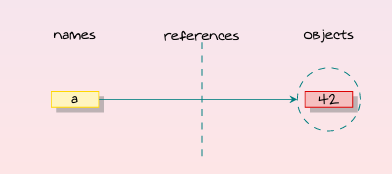
\includegraphics[scale=0.7]{1-variables-object-and-references}
\end{center}

\subsubsection{Types live with objects, not varables}

\begin{lstlisting}[language=Python]
>>> a = 42     # it's an integer
>>> a = 'spam' # now, it's string
>>> s = 3.14   # now, it's a floating point
\end{lstlisting}

\textbf{Coming from typed languages programming}

This lokks as the type of the name a changes

\textbf{Of course, this is not true. In python}

\begin{center}
Name have no types
\end{center}

\textbf{We simply changed the variable reference to a different object}

\textbf{Objects know what type they have}

Each object has an header field that tags it with its type

\textbf{Because objects know their type, variables don't have to}


\subsubsection{Object are garbage collected}

\textbf{What happens to the referenced object when the variable is reassinged?}

\begin{lstlisting}[language=Python]
>>> a = 42     
>>> a = 'spam'  # Reclaim 42 now (unless referenced elsewhere)
>>> s = 3.14    # Reclaim 'spam' now
>>> a = [1,2,3] # Reclaim 3.14 now
\end{lstlisting}

\textbf{The space held by the referenced object is reclaimed (garbage collected)}

If it is not referenced by any other name or object

Automatic garbage collection implies less bookkeeping code

\subsubsection{Shared references}

\textbf{What happens when a name changes its reference and the old valueis still referred?}

\begin{center}
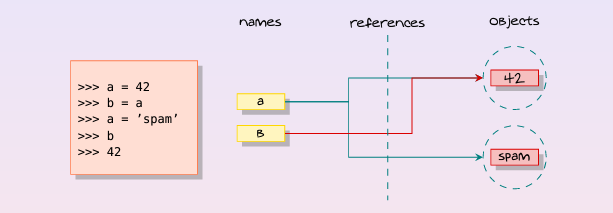
\includegraphics[scale=0.7]{2-shared-references}
\end{center}

\textbf{Is this still the same?}

\begin{lstlisting}[language=Python]
>>> a = [1,2,3]  
>>> b=a
>>> b[1]='spam'
>>> b
[1, 'spam', 3]
>>> a
[1, 'spam', 3]
\end{lstlisting}

\subsubsection{References \& Equality}

\textbf{Two ways to check equality}:

\begin{itemize}
	\item == (equality) and
	item is (object identity)
\end{itemize}

\begin{lstlisting}[language=Python]
>>> L=[1,2,3]
>>> M=[1,2,3]
>>> N=L
>>> L==M L is M
(True, False)
>>> L==N, L is N
(True, True)
\end{lstlisting}


\section{Object Oriented Programming in Python}

Classes, Inheritance & Polymorphism

\subsection{Object-Oriented Programming}

\subsubsection{Introduction}

Python is a multi-paradigm programmin language

Many claims that:

\begin{center}
Python is object-oriented
\end{center}

Python is just \textbf{object-based} but we can use it as if it is object-oriented

Look at

\begin{center}
\textbf{Reference}
Peter Wagner
\textbf{Dimensions of Object-Based Language Design}
In Proceegings of OOPSLA'87, pp. 168-182, October 1987.
\end{center}

for the differences

\subsubsection{Wagner’s OO Taxonomy: Objects, Classes and Inheritance}

\textbf{Objects}
An object has a set of operations and a state that remembers the effect of the operations

\textbf{Class}
A class is a template from which objects may be created

\begin{itemize}
	\item object of the same class have common operations and (therefore) uniform behavior
	\item Class expose a set of operations (public interface) to its clients
\end{itemize}

\textbf{Inheritance}
A class may inherit operations from superclasses and its operations inherited by subclasses

\begin{itemize}
	\item  inheritance can be single or multiple
\end{itemize}

\subsubsection{Wagner’s OO Taxonomy (Cont.’d)}

Wagner suggests 3 classes for programming languages:

\begin{itemize}
	\item object-based = object
	\item class-based = object + classes
	\item object-oriented = onject + classes + inheritance
\end{itemize}

\textbf{Data Abstraction}
A data abstraction is an object whose state is accessible only through its operations

\begin{itemize}
	\iem this concept brings forth to the data hifing property
\end{itemize}

\textbf{Delegation}
Delegation is a mechanism to delegate responsibility for performing an operation to one or more designed ancestors

\begin{itemize}
		\item note that ancestors are not always designed by inheritance in this case it is called clientship
\end{itemize}

\subsubsection{Class Definition: Rectangle}

\begin{lstlisting}[language=Python]
	class rectangle:
		def __init__(self, width, height):
			self._width=width
			self._height=height
		def calculate_area(self):
			return self._width*self._height
		def calculate_perimeter(self):
			return 2*(self._height+self._width)
		def __str__(self):
			return "I’m a Rectangle! My sides are: {0}, {1}\nMy area is {2}".\
			format(self._width,self._height, self.calculate_area())
\end{lstlisting}

\begin{lstlisting}[language=Python]
>>> from rectangle import rectangle
>>> r = rectangle(7,42)
>>> print(r)
I’m a Rectangle! My sides are: 7, 42
My area is 294
\end{lstlisting}

\subsubsection{Inheritance}

Inheritance 



\section{Object Oriented Programming in Python 2}

Part 2: Advance on OOP

\subsection{Object-Oriented Programming}

\subsubsection{Instance vs Class Attributes}

\begin{lstlisting}[language=Python]
class C:
	def __init__(self):
		self.class_attribute="a value"
	def __str__(self):
		return self.class_attribute
\end{lstlisting}

\begin{lstlisting}[language=Python]
[15:18]cazzola@hymir:~/oop>python3
>>> from C import C
>>> c = C()
>>> print(c)
a value
>>> c.class_attribute
'a value'
>>> c1 = C()
>>> c1.instance_attribute = "another value"
>>> c1.instance_attribute
'another value'
>>> c.instance_attribute
Traceback (most recent call last):
File "<stdin>", line 1, in <module>
AttributeError: 'C' object has no attribute 'instance_attribute'
>>> C.another_class_attribute = 42
>>> c1.another_class_attribute, c.another_class_attribute
(42, 42)
\end{lstlisting}

\subsubsection{Alternative Way to Access Attributes: \_\_dict\_\_}

\begin{lstlisting}[language=Python]
>>> c.__dict__
{'class_attribute': 'a value'}
>>> c1.__dict__
{'class_attribute': 'a value', 'instance_attribute': 'another value'}
>>> c.__dict__['class_attribute'] = 'the answer'
>>> print(c)
the answer
\end{lstlisting}

\textbf{\_\_dict\_\_ is an attribute}
\begin{itemize}
	\item it is a dictionary that contains the user-provided attributes
	\item it permits introspection and intercession
\end{itemize}

\textbf{Let’s dynamically change how things are printed}

\begin{lstlisting}[language=Python]
>>> def introspect(self):
... 	result=""
... 	for k,v in self.__dict__.items():
... 		result += k+": "+v+"\n"
... 	return result
...
>>> C.__str__ = introspect
>>> print(c)
class_attribute: the answer
>>> print(c1)
class_attribute: a value
instance_attribute: another value
\end{lstlisting}

\subsection{What about the Methods? Bound Methods}

\begin{lstlisting}[language=Python]
>>> class D:
... 	class_attribute = "a value"
... 	def f(self):
... 		return "a function"
...
>>> print(D.__dict__)
{'__module__': '__main__', 'f': <function f at 0x80bbb6c>,
'__dict__': <attribute '__dict__' of 'D' objects>, 'class_attribute': 'a value',
'__weakref__': <attribute '__weakref__' of 'D' objects>, '__doc__': None}
>>> d = D()
>>> d.class_attribute is D.__dict__['class_attribute']
True
>>> d.f is D.__dict__['f']
False
>>> d.f
<bound method D.f of <__main__.D object at 0x80c752c>>
>>> D.__dict__['f'].__get__(d,D)
<bound method D.f of <__main__.D object at 0x80c752c>>
\end{lstlisting}

\textbf{Functions are not accessed through the dictionary of the class}
	- they must be bound to a an instance

\textbf{A bound method is a callable object that calls a function passing an instance as the first argument}

\subsubsection{Descriptors}

\begin{lstlisting}[language=Python]
class Desc(object):
	"""A descriptor example that just demonstrates the protocol"""
	def __get__(self, obj, cls=None):
		print("{0}.__get({1}, {2})".format(self,obj,cls))
	def __set__(self, obj, val):
		print("{0}.__set__({1}, {2})".format(self,obj,val))
	def __delete__(self, obj):
		print("{0}.__delete__({1})".format(self,obj))

class C(object):
	"A class with a single descriptor"
	d = Desc()
\end{lstlisting}

\begin{lstlisting}[language=Python]
[15:17]cazzola@hymir:~/esercizi-pa>python3
>>> from descriptor import Desc, C
>>> cobj = C()
>>> x = cobj.d # d.__get__(cobj, C)
<descriptor.Desc object at 0x80c610c>.__get(<descriptor.C object at 0x80c3b0c>, <class 'descriptor.C'>)
>>> cobj.d = "setting a value" # d.__set__(cobj, "setting a value")
<descriptor.Desc object at 0x80c610c>.__set__(<descriptor.C object at 0x80c3b0c>, setting a value)
>>> cobj.__dict__['d'] = "try to force a value" # set it via __dict__ avoiding the descriptor
>>> x = cobj.d # this calls d.__get__(cobj, C)
<descriptor.Desc object at 0x80c610c>.__get(<descriptor.C object at 0x80c3b0c>, <class 'descriptor.C'>)
>>> del cobj.d # d.__delete__(cobj)
<descriptor.Desc object at 0x80c610c>.__delete__(<descriptor.C object at 0x80c3b0c>)
>>> x = C.d # d.__get__(None, C)
<descriptor.Desc object at 0x80c610c>.__get(None, <class 'descriptor.C'>)
>>> C.d = "setting a value on class" 
\end{lstlisting}

\subsubsection{Method Resolution Disorder: the Diamond Problem}

\begin{lstlisting}[language=Python]
class A(object):
	def do_your_stuff(self):
		# do stuff for A
		return
\end{lstlisting}

\begin{lstlisting}[language=Python]
class B(A):
	def do_your_stuff(self):
		A.do_your_stuff(self)
		# do stuff for B
		return
\end{lstlisting}

\begin{lstlisting}[language=Python]
class C(A):
	def do_your_stuff(self):
		A.do_your_stuff(self)
		# do stuff for C
		return
\end{lstlisting}

\begin{lstlisting}[language=Python]
class D(B,C):
	def do_your_stuff(self):
		B.do_your_stuff(self)
		C.do_your_stuff(self)
		# do stuff for D
		return
\end{lstlisting}

\textbf{Two copies of A}
\begin{itemize}
	\item if do\_your\_stuff() is called once B or C is incomplete
	\item if called twice it could have undesired side-effects
\end{itemize}

\subsubsection{A Pythonic Solution: The "Who's Next" List}
\textbf{The solution is to dynamically determine which do\_your\_stuff() to call in each do\_your\_stuff()}

\begin{lstlisting}[language=Python]
B.next_class_list = [B,A]
C.next_class_list = [C,A]
D.next_class_list = [D,B,C,A]

class B(A):
	def do_your_stuff(self):
		next_class = self.find_out_whos_next(B)
		next_class.do_your_stuff(self)
		# do stuff with self for B
	def find_out_whos_next(self, clazz):
		l = self.next_class_list # l depends on the actual instance
		mypos = l.index(clazz) # Find this class in the list
		return l[mypos+1] # Return the next one
\end{lstlisting}

\textbf{find\_out\_whos\_next() depends on who we are working with}
- B.do() -> B.find(B) -> l = [B,A] ->  l[index(B)+1=1] = A ->  A.do()
- D.do() -> D.find(D) -> l = [D,B,C,A] -> l[index(D)+1=1] = B -> B.do()
         -> B.find(B) -> l = [D,B,C,A] -> l[index(B)+1=2] = C -> C.do()
         -> C.find(C) -> l = [D,B,C,A] -> l[index(C)+1=3] = A -> A.do()

do() = do\_your\_stuff() find(...) = find\_out\_whos\_next(...)

\subsubsection{\_\_mro\_\_ \& super}
\textbf{There are a class attribute \_\_mro\_\_ for each type and a super}
\begin{itemize}
	\item \_\_mro\_\_ keeps the list of the superclasses without duplicates in a
predictable order
	\item super is used in place of the find\_out\_whos\_next()
\end{itemize}

\begin{center}
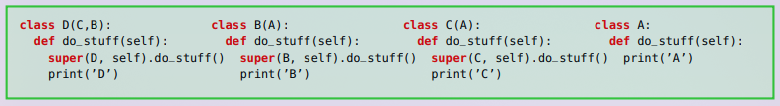
\includegraphics[scale=0.7]{3-OOP-1}
\end{center}

\textbf{Computing the method resolution order (MRO)}
\begin{itemize}
	\item if A is a superclass of B then B>A
	\item if C precedes D in the list of bases in a class statement then C>D
	\item if E>F in one scenario then E>F must hold in all scenarios
\end{itemize}

\begin{lstlisting}[language=Python]
[23:04]cazzola@hymir:~/esercizi-pa>python3
>>> from mro import A,B,C, D
>>> D.__mro__
(<class 'mro.D'>, <class 'mro.C'>, <class 'mro.B'>, <class 'mro.A'>, <class 'object'>)
>>> d = D()
>>> d.do_stuff()
A
B
C
D
\end{lstlisting}

\subsubsection{Special Methods}

\textbf{Special methods, as \_\_len\_\_(), \_\_str\_\_(), \_\_lt\_\_() and \_\_add\_\_(),
govern the behavior of some standard operations}

\begin{lstlisting}[language=Python]
class C(object):
	def __len__(self):
		return 0
def mylen():
	return 1
\end{lstlisting}

\begin{lstlisting}[language=Python]
[10:03]cazzola@hymir:~/pa>python3
>>> cobj = C()
>>> cobj.__len__ = mylen
>>> len(cobj)
0
\end{lstlisting}

\textbf{Special methods are “class methods”}
\begin{itemize}
	\item they cannot be changed through the instance
	\item this goes straight to the type by calling C.\_\_len\_\_()
\end{itemize}

\begin{lstlisting}[language=Python]
class C(object):
	def __len__(self): return self._mylen()
	def _mylen(self): return 0
def mylen():
	return 1
\end{lstlisting}

\begin{lstlisting}[language=Python]
[10:22]cazzola@hymir:~/pa>python3
>>> cobj = C()
>>> cobj._mylen = mylen
>>> len(cobj)
1
\end{lstlisting}

\textbf{To be more flexible}
- the special method must be forwarded to a method that can be overridden in the instance

\subsubsection{\_\_slots\_\_}

\textbf{Also built-in types, as list and tuple, can be subclassed}

\begin{lstlisting}[language=Python]
class MyList(list):
	"""A list that converts added items to ints"""
	def append(self, item):
		list.append(self, int(item))
	def __setitem__(self, key, item):
		list.__setitem__(self,key,int(item))
\end{lstlisting}

\begin{lstlisting}[language=Python]
[10:45]cazzola@hymir:~/esercizi-pa>python3
>>> l = MyList()
>>> l.append(1.3)
>>> l.append(444)
>>> l
[1, 444]
>>> len(l)
2
>>> l[1] = 3.14
>>> l
[1, 3]
\end{lstlisting}

\textbf{Unfortunately the subtype of list allow the adding of attributes}
- this is due to the presence of \_\_dict\_\_

\textbf{The presence of \_\_slots\_\_ in a class definition inhibits the introduction of \_\_dicts\_\_}
- this disallows any user-define attributes

\begin{lstlisting}[language=Python]
class MyList2(list):
	__slots__ = []
class MyList3(list):
	__slots__ = ['color']
class MyList4(list):
	"""A list that contains only ints"""
	def __init__(self, itr):
		list.__init__(self, [int(x) for x in itr])
	def append(self, item):
		list.append(self, int(item))
	def __setitem__(self, key, item):
		list.__setitem__(self,key,int(item))
\end{lstlisting}


\begin{lstlisting}[language=Python]
[11:13]cazzola@hymir:~/esercizi-pa>python3
>>> m2 = MyList2()
>>> m2.color = 'red'
Traceback (most recent call last):
File "<stdin>", line 1, in <module>
AttributeError:
'MyList2' object has no attribute 'color'
>>> m3 = MyList3()
>>> m3.color = 'red'
>>> m3.weight = 50
Traceback (most recent call last):
File "<stdin>", line 1, in <module>
AttributeError:
'MyList3' object has no attribute 'weight'
\end{lstlisting}

\end{document}
